\documentclass[prd,twocolumn,superscriptaddress,nofootinbib,amsmath,amssymb,floatfix]{revtex4-2}
\usepackage{graphicx}
\usepackage{xcolor}
\graphicspath{{../figs/}}
\usepackage{booktabs}
\usepackage[colorlinks=true,linkcolor=blue!50!black,citecolor=blue!50!black,urlcolor=blue!50!black]{hyperref}
\newcommand{\pending}[1]{\textcolor{red}{[#1]}}

% 3+1 paper, split from counting-full-v2.tex (session 15, 2026-10-29). Companion: toolkit-1p1-v1.tex; methodology: methodology-note-v1.tex.
% Rules (Roberto): PRD register; failed attempts only in App. A (deletable); AI use = short disclosure + citation of the methodology note.
% Round 2 (referee agent): low-count claim now tested on Johnston's own detours (r30); per-pair errors (r29); sets of universes labelled; correlation renamed C.
% v2 (session 17, external referee round 1, answer in ~/Desktop/papers/3+1 PRD/answers/answer-embedding-3p1-v2.md): 10 universes per size up to 6000 (r35);
% Casasola near-cone ablation, optimizer check (L-BFGS, three starts), joint time-space fit (r35); significance paragraph; ESV19 / MRS06 / MRS07;
% table of sprinkling sets; error-location figure; abstract trimmed. Correction: the residual is NOT an optimizer effect (v1 said "local optimum").

\begin{document}

\title{Spatial embedding of $3+1$ causal sets: low-count spacelike pairs and a likelihood fit to interval counts}

\author{Roberto Bada}
\email{roberto@sapereia.com}
\affiliation{SapereIA, Barcelona, Spain}
\affiliation{Institute of Cosmos Sciences, University of Barcelona (ICCUB), Barcelona, Spain}

\date{\today}

\begin{abstract}
Recovering spatial distances from the causal order alone is a central open problem in the kinematics of causal sets. We study it on the benchmark of Johnston's recent embedding of $3+1$ causal sets into Minkowski spacetime [Phys.\ Rev.\ D \textbf{111}, 106020 (2025)]. With oracle substitutions we show that almost all of the residual error of that method comes from spacelike pairs whose shared causal regions contain fewer than ten elements; these pairs concentrate at the waist of the causal diamond and become rarer only slowly with density. We therefore fit the spatial coordinates to the interval counts of related pairs with a Poisson likelihood (Casasola's), starting from a map built from causal-overlap counts alone. On $44$ sprinklings with $1000$--$15000$ elements the fit improves on Johnston's embedding in every universe, removes three quarters to four fifths of his residual, and roughly halves the typical error of individual spatial distances. The remaining error is set by directions in which the likelihood is nearly flat, not by the optimizer. In a region without a waist the gain is smaller, because intervals are truncated at its timelike boundary.
\end{abstract}

\maketitle

\section{Introduction}\label{sec:intro}
In causal set theory spacetime is modeled as a locally finite partially ordered set, whose elements are spacetime events and whose order is the causal order~\cite{BLMS87,Surya19}. For a causal set obtained by a Poisson sprinkling into a Lorentzian manifold, the number of elements in a region estimates its spacetime volume, and the order encodes the light cones; the kinematic programme is to recover the remaining geometry from these two ingredients. Timelike quantities are comparatively accessible: the longest chain between two related elements estimates their proper time~\cite{BrightwellGregory91}, and interval counts give dimension and curvature~\cite{GlaserSurya13,RSS13,BD10}. Spatial distances are harder, because two spacelike elements bound no interval.

Several constructions address this. Brightwell and Gregory and, in more detail, Rideout and Wallden defined spatial distance through intervals between common past and future elements~\cite{BrightwellGregory91,RideoutWallden09}. Major, Rideout and Surya represented spatial hypersurfaces by thickened antichains and recovered their topology from the order~\cite{MRS06,MRS07}; Eichhorn, Surya and Versteegen defined distances on such hypersurfaces from the volume of the smallest common future of two elements, minimized over paths with a mesoscale cutoff, and showed that, because no element is exactly null related to another, short distances are overestimated (``discrete asymptotic silence'')~\cite{ESV19}. Bogu\~n\'a and Krioukov measured spatial distance through the overlap of the causal pasts of two elements as seen from a common past element~\cite{BK24}, and Hu, Meyer and Meyer gave an exact $1+1$ reconstruction~\cite{HMM25}. Embeddings of whole causal sets into Minkowski spacetime were constructed by Henson~\cite{Henson06}, by Clough and Evans through Lorentzian multidimensional scaling~\cite{CloughEvans16}, and by Johnston, first through factorization of matrices of inner products~\cite{Johnston22} and recently through a simpler method~\cite{Johnston25} that is the current benchmark for $3+1$ sprinklings into a causal diamond. In that method the spatial separation of a spacelike pair is the shortest detour through an element related to both.

Why the accuracy of a flat embedding matters is worth stating, because the benchmark itself is flat. First, coordinates are the input of most further geometric constructions on a causal set: spatial distances on hypersurfaces~\cite{ESV19}, local charts from which curvature is reconstructed~\cite{Madsen26}, and the comparison of discrete fields with their continuum counterparts at the positions of elements. Second, embedding tests of manifoldlikeness~\cite{CloughEvans16,Toolkit} can only reject a causal set when the embedding error on a genuine sprinkling is small compared with the misfit of a non-manifoldlike one, so a less noisy embedding is a sharper test. Third, and independent of any method, locating the residual error tells us which information the order carries poorly: we find that it is the spacelike pairs with few shared elements, the same pairs whose distances are overestimated in the construction of Ref.~\cite{ESV19}. We do not demonstrate a downstream application in this paper; the claims concern accuracy on the benchmark and the source of its error.

In this paper we ask where the remaining error of Johnston's embedding comes from, and how to remove it. Our results are the following.
\begin{enumerate}
\item We reproduce his benchmark and show by oracle substitution that the residual error is entirely due to spacelike pairs, and almost entirely due to those whose shared causal regions contain fewer than ten elements (Secs.~\ref{sec:johnston} and~\ref{sec:overlap}).
\item With a causal-overlap distance estimator built on Bogu\~n\'a and Krioukov's construction, extended to reference elements at unequal depth, we show that these low-count pairs also limit the classical-scaling embedding of inverted distances, and give a scaling argument for why their errors decrease only slowly with density (Sec.~\ref{sec:overlap}).
\item We fit the spatial coordinates directly to the interval counts of related pairs, with their Poisson noise. The likelihood is Casasola's~\cite{Casasola26}; our contributions are an intrinsic starting map, a controlled comparison with Ref.~\cite{Johnston25} up to $n=15000$, where the fit removes three quarters to four fifths of the residual error, and ablations showing which ingredients matter and that the remaining error is a property of the likelihood, not of the optimizer (Sec.~\ref{sec:likelihood}).
\item We repeat the comparison in a region without a waist at equal density, and identify the timelike boundary as the source of the reduced gain (Sec.~\ref{sec:slab}).
\end{enumerate}
The cost of the methods is compared in Sec.~\ref{sec:cost}, and Sec.~\ref{sec:disc} discusses novelty, limitations and extensions. Other approaches that we tested are summarized in Appendix~\ref{app:dropped}. A companion paper develops exact counting tools in $1+1$ dimensions~\cite{Toolkit}.

\section{Setup and benchmark}\label{sec:setup}
Following Ref.~\cite{Johnston25}, a Poisson number of points with mean $n$ is sprinkled with density $\rho$ into a causal diamond of height $1$ in $3+1$ Minkowski spacetime (waist radius $\tfrac12$, volume $\pi/24$), and the bottom and top tips $v_1,v_n$ are added as two further elements. The order is induced by the light cones; the coordinates are then discarded and used only for scoring. We write $\ell=\rho^{-1/4}$ for the discreteness length, so that a region of volume $\ell^4$ contains one element on average; at $n=3000$ the diamond height is $\approx 12\,\ell$. For a related pair $a\prec b$, $N_{ab}$ denotes the number of elements strictly between them; in a flat interval of proper time $\tau$ its mean is $\rho\,\pi\tau^4/24$.

A method returns coordinates from the order alone. As in Table~V of Ref.~\cite{Johnston25}, the score is the Pearson correlation $\mathcal C$ between embedded and true spatial distances over all pairs. We report the residual $1-\mathcal C$ and, for a new method, the fraction of Johnston's residual that it removes, $(\mathcal C-\mathcal C_{\rm J})/(1-\mathcal C_{\rm J})$, always on the same universes. Because a correlation close to one is dominated by distant pairs and insensitive to an overall rescaling, we also report per-pair distance errors and position errors in units of $\ell$ (Sec.~\ref{sec:likelihood}).

Table~\ref{tab:sets} lists the sets of sprinklings; every number below states which set it comes from. Quoted uncertainties are standard errors over universes.

\begin{table}[t]
\caption{Sets of sprinklings. Time coordinate: Johnston's (J) or the true one (true). All sets use independent seeds; the large-$n$ set at $n\le6000$ contains the universes of v1 of this paper.}
\label{tab:sets}
\begin{ruledtabular}
\begin{tabular}{llcc}
set & $n$ (universes) & time & used in\\
\hline
development & $500$--$1500$ ($10$ per $n$), $400$--$2000$ & J/true & Sec.~\ref{sec:johnston}, check (i)\\
diagnostic & $1500$ (3), $3000$ (2) & J & Sec.~\ref{sec:overlap}\\
check & $1500$ (3), $3000$ (2) & J & checks (ii), (iv)\\
large-$n$ & $1000$, $3000$, $6000$ (10 each),\\
 & $10000$ (8), $15000$ (6) & J & Sec.~\ref{sec:likelihood}, Fig.~\ref{fig:3p1}\\
shape & diamond $1500$, $3000$; slab $1500$, & true & Sec.~\ref{sec:slab}\\
 & $6000$, $12000$ (3--4 each) & & \\
\end{tabular}
\end{ruledtabular}
\end{table}

\section{Johnston's embedding}\label{sec:johnston}
Johnston assigns each element a time coordinate from volumes and the proper time of related pairs from interval counts, so that the spatial separation of a related pair is $R=\sqrt{\Delta t^2-\tau^2}$. For a spacelike pair he takes the shortest detour through an element $z$ related to both,
\begin{equation}
r(x,y)=\min_z\big[R(x,z)+R(z,y)\big],
\label{eq:detour}
\end{equation}
an upper bound by the triangle inequality, computed as a min-plus matrix product. Classical multidimensional scaling of $r$ then gives three spatial coordinates.

Our implementation reproduces his Table~V, $\mathcal C=0.786$, $0.887$, $0.923$ at $n=500$, $1000$, $1500$ (ten sprinklings each) against his $0.789$, $0.887$, $0.928$, and his Table~III, provided the proper time is computed from the elements strictly between the two endpoints; including the endpoints gives $\mathcal C=0.72$ at $n=1000$, as also noted by Pellegrin~\cite{Pellegrin26}. For the correlation of squared Minkowski intervals (his Table~IV) we obtain $0.82$, $0.90$, $0.93$ against his $0.958$, $0.977$, $0.985$, also when the true time coordinate is used; we suspect that a different statistic is reported there, and use the spatial correlation throughout.

On development sprinklings, replacing the spacelike values $r$ by the true spatial distances, and keeping every other step, raises $\mathcal C$ from $0.903$ to $0.9999$ at $n=1000$ (from $0.915$ to $0.9999$ at $n=1500$). Replacing instead the related-pair separations by their true values leaves it essentially unchanged ($0.903\to0.906$). The residual error of the method therefore resides in the spacelike pairs. Pellegrin, studying a link-restricted version of the detour, attributes much of its error to noisy related-pair distances of near-collinear pairs~\cite{Pellegrin26}; for Eq.~\eqref{eq:detour} itself, correcting the related pairs does not help.

\section{Overlap distances and low-count pairs}\label{sec:overlap}
\emph{Estimator.} Let $a,b$ be spacelike and $c$ an element in their common past. In flat spacetime the volumes of $I(c,a)$, $I(c,b)$ and of their overlap $C$ depend only on the proper times $\tau_{ca}\geq\tau_{cb}$ and on the spatial distance $d$. The overlap in units of the smaller interval,
\begin{equation}
w=\frac{V_C}{V_b}=w\!\left(\frac{\tau_{cb}}{\tau_{ca}},\frac{d}{\tau_{ca}}\right)\in[0,1],
\end{equation}
depends on two ratios only. We tabulate it once by Monte Carlo integration ($\tau_{cb}/\tau_{ca}\in[0.05,1]$, $d/\tau_{ca}\le8$, common random numbers) and invert it in $d$, reading both proper times from interval counts through $V=\pi\tau^4/24$. On the causal set we use $w=(N_C+\tfrac12)/(N_b+1)$, which keeps the inversion finite at $N_C=0$, and cap the result at the detour of Eq.~\eqref{eq:detour}, an upper bound for exact separations. For the benchmark we take $c=v_1$, so that $d(a,b)$ requires only the sizes of the two pasts and of their intersection, and we use the future side ($c=v_n$) when it contains more elements. These counts for all pairs follow from two matrix products. The same three counts define M\"uller's past-cone metric~\cite{Muller25}, without an inversion to a distance.

This is the construction of Bogu\~n\'a and Krioukov~\cite{BK24}, who introduced the overlap of two causal intervals with a common past element as a measure of spatial distance and proposed embedding the resulting distance matrix. They invert the overlap exactly, numerically and in any dimension, for $c$ at equal proper time below $a$ and $b$ [their Eq.~(22)], and on a causal set keep only reference elements at equal depth [their Eqs.~(32)--(34)]. Our extension is the table for unequal depths, $\tau_{cb}/\tau_{ca}<1$, which allows a single reference element for all pairs. The Euclidean analogue, the distance between two sensors from the numbers of shared and unshared neighbors, is known in sensor-network localization, both as a deterministic inversion~\cite{Buschmann06} and as a maximum-likelihood estimate with a Cram\'er--Rao bound~\cite{Huang14}. For late elements of large sprinklings ($n=2\times10^4$--$8\times10^4$), whose shared pasts are large, the estimator has a median relative error of $1$--$2\%$ and a bias below $1\%$ for $d\geq4\ell$, and $6$--$8\%$ below $2\ell$.

\emph{Per pair and as an embedding.} On the benchmark most pairs are not late, and the counts are much smaller. Table~\ref{tab:profile} compares the two estimates over all spacelike pairs, by true separation. The detour is poor for close pairs, where no element lies between them (its $+40\%$ bias below $0.1$ is the overestimate of short distances described in Ref.~\cite{ESV19}), and accurate for distant pairs, where many elements lie near the straight line; the overlap estimate behaves in the opposite way and is biased low by $5$--$17\%$. Restricted to pairs with at least $20$ elements in the shared region, its median per-pair error is lower than that of the detour ($0.112$ against $0.132$ at $n=1000$; $0.062$ against $0.083$ at $n=3000$). As a diagnostic, we embed the overlap estimates directly by classical scaling: the result is much worse than Johnston's ($1-\mathcal C=0.18$ against $0.049$ at $n=3000$; Fig.~\ref{fig:3p1}). Per-pair accuracy does not translate into an accurate embedding.

\begin{table}[t]
\caption{Spacelike spatial distances by true separation, $n=1500$ (all spacelike pairs of one universe): median signed bias and median absolute relative error of the overlap estimate and of Johnston's detour, Eq.~\eqref{eq:detour}.}
\label{tab:profile}
\begin{ruledtabular}
\begin{tabular}{lrcccc}
true $|\Delta\mathbf x|$ & pairs & \multicolumn{2}{c}{overlap} & \multicolumn{2}{c}{detour}\\
 & & bias & error & bias & error\\
\hline
$0$--$0.1$ & 3\,872 & $-0.05$ & $0.16$ & $+0.40$ & $0.48$\\
$0.1$--$0.2$ & 43\,341 & $-0.16$ & $0.21$ & $-0.08$ & $0.34$\\
$0.2$--$0.35$ & 217\,706 & $-0.17$ & $0.18$ & $-0.12$ & $0.22$\\
$0.35$--$0.5$ & 295\,991 & $-0.14$ & $0.15$ & $-0.07$ & $0.13$\\
$0.5$--$1$ & 230\,652 & $-0.11$ & $0.12$ & $+0.01$ & $0.06$\\
\end{tabular}
\end{ruledtabular}
\end{table}

\emph{Low-count pairs.} Let $k$ be the number of elements in the shared region on the side used by the overlap estimator. Pairs with $k<10$ are $50\%$ of the spacelike pairs at $n=1500$ and $31\%$ at $n=3000$; most of them straddle the waist of the diamond, where both the common past and the common future are small. A second oracle locates Johnston's error on them (diagnostic sets): replacing his detour by the true distance on the $k<10$ pairs only removes $97\%$ ($n=1500$) and $94\%$ ($n=3000$) of his residual, while the truth on all other spacelike pairs removes $3\%$ and $4\%$ ($97$--$99\%$ against $2\%$ with the threshold $k<30$). The same holds for the overlap estimates on the same universes: with the truth on the $k<10$ pairs, their direct embedding removes $96\%$ ($n=1500$) and $88\%$ ($n=3000$) of Johnston's residual, while the truth on all other pairs leaves it far worse than his. Classical scaling gives the noisy low-count distances the same weight as all others, whichever estimator supplies them.

\emph{Why higher density helps slowly.} The distance is carried by the elements in the past of $b$ that are not in the past of $a$. For small $d$ this region is a shell of thickness $\sim d$ on a cone of height $\tau$, containing $\kappa\rho\,d\,\tau^3$ elements with $\kappa=O(1)$. Its Poisson fluctuation gives, as an order-of-magnitude estimate,
\begin{equation}
\frac{\delta d}{d}\sim\frac{1}{\sqrt{\kappa\rho\,d\,\tau^3}}.
\label{eq:dd}
\end{equation}
At fixed shape all lengths grow as $n^{1/4}$ in units of $\ell$, so $d\tau^3\propto n$ and $\delta d/d\propto n^{-1/2}$ for a typical pair; the measured median errors fall as $n^{-0.54}$ (overlap) and $n^{-0.42}$ (detour) between $n=1000$ and $3000$. The tail, however, is geometric: a pair on opposite sides of the waist has a small common past \emph{and} a small common future, so its $\tau$ in Eq.~\eqref{eq:dd} is set by its position rather than by the density. Between $n=6000$ and $15000$, the range least affected by small-$n$ effects, the residual of the direct overlap embedding falls approximately as $n^{-0.4}$, against $n^{-0.85}$ for Johnston's (large-$n$ set, Fig.~\ref{fig:3p1}); between $n=3000$ and $6000$ it still halves. This motivates using the counts themselves, with their noise, instead of distances inverted from them.

\section{Fitting coordinates to interval counts}\label{sec:likelihood}
\emph{Likelihood.} We keep Johnston's time coordinates $t_i$ and treat the $3n$ spatial coordinates $\mathbf x_i$ as unknowns. For a related pair $a\prec b$, $N_{ab}$ is Poisson-distributed with mean $\rho\,\pi\tau_{ab}^4/24$, where $\tau_{ab}^2=(t_b-t_a)^2-|\mathbf x_b-\mathbf x_a|^2$. We use this in Gaussian form for $\tau^2$: with
\begin{equation}
\widehat{\tau^2}_{ab}=\Big(\frac{N_{ab}+\tfrac12}{\rho\pi/24}\Big)^{1/2},\qquad s_{ab}=\frac{\widehat{\tau^2}_{ab}}{2\,\big(N_{ab}+1\big)^{1/2}},
\end{equation}
which corresponds to a relative error $\delta N/2N$ (the shifts $\tfrac12$ and $1$ keep pairs with $N_{ab}=0$ finite),
\begin{equation}
\ln L(\mathbf x)=-\frac12\sum_{a\prec b}\left(\frac{\tau^2_{ab}(\mathbf x)-\widehat{\tau^2}_{ab}}{s_{ab}}\right)^{2},
\label{eq:lik}
\end{equation}
summed over all related pairs (whether all are needed is tested below). Spacelike pairs do not enter. Each element is constrained by its $O(n)$ related partners, a pair with many elements between it tightly and one with few loosely; this is the weighting that classical scaling lacks. The Gaussian form is a convenience: the exact Poisson log-likelihood $\sum[N\ln\mu-\mu]$ gives the same maps (check (iv) below), provided it also encodes that the pair is related; otherwise a pair with $N=0$ is best fitted as spacelike at no cost, and the fit drifts. The Gaussian form, whose target $\widehat{\tau^2}$ is always positive, needs no such term. We maximize Eq.~\eqref{eq:lik} with the Adam optimizer and the analytic gradient (checked against finite differences), for 400 iterations with a step of $1\%$ of the spatial spread, reduced by a factor $0.3$ halfway; the tips are fixed at $\mathbf x=0$. Each iteration costs $O(\#\text{related pairs})=O(n^2)$.

\emph{Starting map.} The fit requires a start that is roughly correct and is itself derived from the order. We embed the overlap estimates of Sec.~\ref{sec:overlap} by weighted stress majorization (SMACOF~\cite{deLeeuwMair09}; accuracy-weighted scaling is standard in sensor localization~\cite{CostaPatwariHero06}), with weight $k/(k+100)$ for each spacelike pair and $1$ for each related pair, so that low-count distances have little influence. This map alone removes $23$--$59\%$ of Johnston's residual, less at large $n$ (Table~\ref{tab:lik}).

\emph{Relation to previous work.} Fitting causal-set coordinates to interval counts with a Poisson likelihood was proposed by Casasola~\cite{Casasola26}, who used a pseudo-likelihood $\sum[N\ln\mu-\mu]$ over related pairs near the light cone ($\tau^2<6\ell^2$) in a $3+1$ diamond, with Langevin sampling started from the \emph{true} positions displaced by about $\ell$; an intrinsic start was left as an open problem, and no comparison with Ref.~\cite{Johnston25} was made. Maximum-likelihood coordinates are standard in other contexts: multidimensional scaling~\cite{Ramsay77}, latent-space network models~\cite{Hoff02}, hyperbolic maps of complex networks, including a geometric first guess refined by likelihood as here~\cite{BPK10,Mercator19}, and directed graphs in Minkowski space~\cite{Sim21}. What we add is the intrinsic start, the large-$n$ test on Johnston's benchmark, and the ablations below. Casasola's preprint has not been peer reviewed; we take from it the form of the likelihood and the near-cone set of pairs, and reproduce both here.

\emph{Results.} Table~\ref{tab:lik} and Fig.~\ref{fig:3p1} show the fit on the large-$n$ set, paired with Johnston's embedding on the same universes. The fit improves on his embedding in each of the $44$ universes. It removes $72\%$ of his residual at $n=1000$, $74\%$ at $n=3000$, $80\%$ at $n=6000$, and $79$--$83\%$ at $n=10000$ and $15000$; across the ten universes of each size up to $6000$ the removed fraction ranges from $61$ to $85\%$ (standard deviation $7$, $6$ and $3$ percentage points at $n=1000$, $3000$, $6000$). The removed fraction rises at most slowly with $n$, so the gap does not close. At $n=15000$ the spatial correlation is $0.9980$ against $0.9886$. The oracle value with exact spacelike distances, $0.9999$, remains higher.

\emph{Per-pair errors and causal fidelity.} In units of the discreteness length, the median absolute error of the embedded spatial distances is $0.33$, $0.23$, $0.18$ for Johnston's embedding and $0.20$, $0.14$, $0.12$ for the fit at $n=1000$, $3000$, $6000$ (ten universes each); the $90$th percentiles are $1.14$, $0.76$, $0.59$ against $0.46$, $0.33$, $0.27$, and the $99$th $3.1$, $2.9$, $2.4$ against $1.4$, $0.6$, $0.5$. Spacelike pairs do not enter Eq.~\eqref{eq:lik}, so we checked how much of the order the fitted coordinates reproduce: the fit misclassifies $1.24\%$, $0.68\%$ and $0.48\%$ of all pairs (related as spacelike or vice versa), against $3.3\%$, $1.7\%$ and $1.1\%$ for Johnston's embedding.

\emph{Where the error remains.} Figure~\ref{fig:errloc} shows the rms position error per element, after removing the best orthogonal map, against the number of related partners of the element and against its time. In both embeddings the error is concentrated on the tenth of the elements with the fewest related partners and, in time, at the waist ($t\approx\tfrac12$); the fit lowers it at every decile and every time, but these elements remain the largest contribution. The rms position error therefore improves less than the median ($0.67\to0.52\,\ell$ at $n=3000$, in the two universes of this size analysed in version 1): the tenth of the elements with the fewest related partners carries an rms of $1.4$--$1.6\,\ell$ in the fit, the other nine tenths $0.18$--$0.19\,\ell$. Neither a global rescaling nor an affine map removes this part.

\emph{Is the residual set by the optimizer?} No. Adam is not fully converged after 400 iterations: continuing with L-BFGS raises the log-likelihood by $45$ on average at $n=3000$ (up to $98$) and by $176$ at $n=6000$ (up to $410$), but changes $\mathcal C$ by only $+1\times10^{-4}$ and $+2\times10^{-4}$. Started from the intrinsic map, from Johnston's map, or from the intrinsic map with every coordinate displaced by $0.5\,\ell$, and run to convergence, the fit reaches the same log-likelihood within a few units out of $4.7\times10^5$ terms at $n=3000$ (within $10$ out of $1.9\times10^6$ at $n=6000$), and the same $\mathcal C$ within the spread between universes (Johnston's start: $+0.0007\pm0.0005$ at $n=3000$, $-0.0003\pm0.0005$ at $n=6000$; choosing the start with the highest likelihood: $75.4\%$ instead of $74.5\%$ at $n=3000$, $81.0\%$ instead of $80.6\%$ at $n=6000$). Started from the true positions (with Johnston's time coordinate), the fit stays much closer to the truth ($\mathcal C=0.9965$, $92\%$ of the residual removed at $n=3000$), yet its log-likelihood exceeds that of the converged intrinsic fit by only $0.9$ on average (at most $5$; at $n=6000$, where the truth-started fit removes $93\%$, by $2.3$, at most $6.5$). The two maps are therefore equally consistent with the counts: the residual is set by directions in which the likelihood is nearly flat, mainly the positions of weakly constrained elements, not by the optimizer. (Version 1 of this paper attributed the residual to a local optimum, because Adam had not converged; that conclusion was wrong.)

\emph{Which pairs are needed?} Casasola restricted the likelihood to pairs near the light cone~\cite{Casasola26}. We ran his exact Poisson form, with the soft relation term of check (iv), once on all related pairs and once on the pairs with $\widehat{\tau^2}<6\,\ell^2$ only ($64\%$, $47\%$ and $37\%$ of related pairs at $n=1000$, $3000$, $6000$), from the same intrinsic start. The near-cone version is slightly better: $\Delta\mathcal C=+0.0004$ at $n=3000$, in ten of ten universes, and $+0.0003$ at $n=6000$, again in ten of ten; the Gaussian form restricted to the same pairs gives $+0.0002$. Distant related pairs therefore add no information that the fit uses, and using all related pairs, which version 1 of this paper listed as a contribution, is not one. The near-cone set also lowers the cost per iteration by a factor of two to three.

\emph{Time coordinate.} The fit keeps Johnston's time coordinate. Fitting the time coordinates jointly with the spatial ones (the tips fixed, same likelihood, Adam and L-BFGS) changes $\mathcal C$ by $+0.0004\pm0.0001$ at $n=3000$ and $+0.0002\pm0.0001$ at $n=6000$ and does not reduce the time error ($0.074$ against $0.076\,\ell$ rms at $n=3000$, $0.062$ against $0.066\,\ell$ at $n=6000$): Johnston's time coordinate is already accurate to a tenth of a discreteness length, and the related-pair counts do not improve it.

\begin{table}[t]
\caption{Likelihood fit, Eq.~\eqref{eq:lik}, against Johnston's embedding on the large-$n$ set, paired on the same universes. Gain: $\mathcal C-\mathcal C_{\rm J}$ with the standard error of the paired differences in parentheses. Last three columns: fraction of Johnston's residual removed by the fit (mean, and range over universes) and by its starting map. Rows $n\le6000$: runs of this version (\texttt{r35}); $n\ge10000$: version 1.}
\label{tab:lik}
\begin{ruledtabular}
\begin{tabular}{rccccccc}
$n$ & univ. & $\mathcal C_{\rm J}$ & $\mathcal C$ (fit) & gain & fit & range & start\\
\hline
1000 & 10 & 0.8855 & 0.9678 & $0.082(14)$ & 72\% & 61--81\% & 59\%\\
3000 & 10 & 0.9551 & 0.9884 & $0.0334(19)$ & 74\% & 64--81\% & 43\%\\
6000 & 10 & 0.9764 & 0.9953 & $0.0189(7)$ & 80\% & 76--85\% & 33\%\\
10000 & 8 & 0.9846 & 0.9968 & $0.0122(3)$ & 79\% & & 23\%\\
15000 & 6 & 0.9886 & 0.9980 & $0.0094(2)$ & 83\% & & 26\%\\
\end{tabular}
\end{ruledtabular}
\end{table}

\begin{figure}[t]
\centering
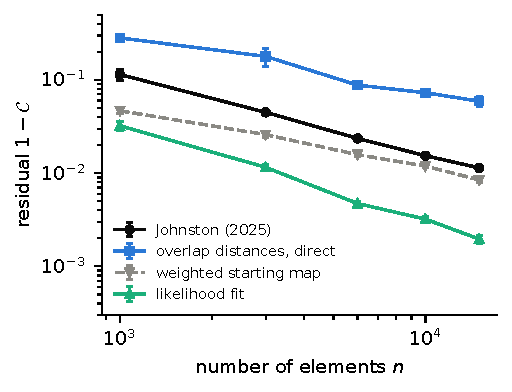
\includegraphics[width=\columnwidth]{fig_3p1_prd_v2}
\caption{Residual $1-\mathcal C$ of the spatial-distance correlation on Johnston's benchmark (large-$n$ set; $n=10^3$--$1.5\times10^4$ with 10, 10, 10, 8 and 6 universes; the overlap-distance curve uses the 1, 2, 4, 8, 6 universes of version 1): his embedding~\cite{Johnston25}, the direct embedding of overlap distances (Sec.~\ref{sec:overlap}), the weighted starting map, and the likelihood fit, Eq.~\eqref{eq:lik}. Error bars: standard error over universes.}
\label{fig:3p1}
\end{figure}

\begin{figure}[t]
\centering
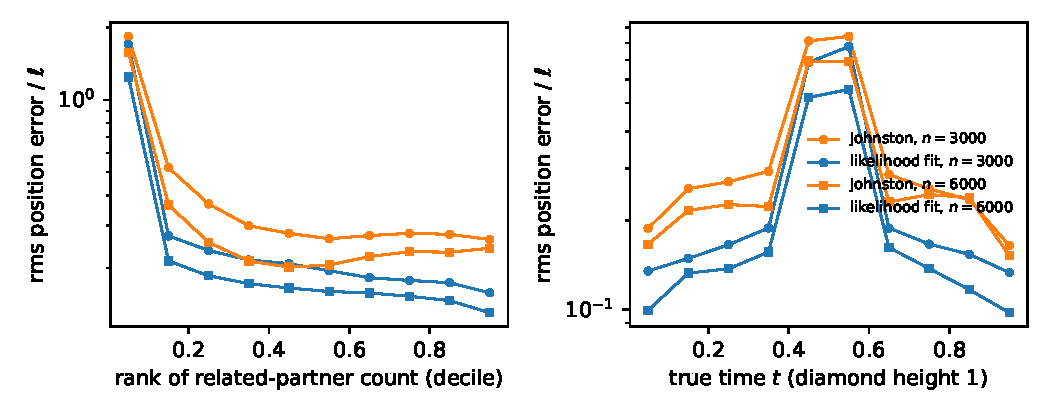
\includegraphics[width=\columnwidth]{fig_3p1_errloc}
\caption{Where the error remains: rms position error per element (after the best orthogonal map), in units of $\ell$, for Johnston's embedding and the likelihood fit (converged), large-$n$ set at $n=3000$ and $6000$ (ten universes each). Left: by decile of the element's number of related partners. Right: by true time.}
\label{fig:errloc}
\end{figure}

\emph{Checks.} (i) \emph{Consistency.} Started from the true positions (with true times), the fit departs from the truth only by finite-$n$ noise and approaches it as $n$ grows: $\mathcal C=0.966$, $0.991$, $0.9965$ at $n=400$, $1000$, $2000$. (ii) \emph{Start independence}, shown above on the large-$n$ set. (iii) \emph{No tuning on the test universes.} The large-$n$ runs used settings fixed beforehand on other universes, including the start's weight scale $100$. (iv) \emph{Form of the likelihood and convergence.} On the check sets we compared the Gaussian form with the exact Poisson log-likelihood plus a soft relation term $\sum\ln\mathrm{sig}(\tau^2/s_0)$, with $\mathrm{sig}$ the logistic function and $s_0=0.1\,\ell^2$ (cf.\ the soft walls of Ref.~\cite{Casasola26}), each at 400 and 1000 iterations. All four variants remove $76$--$77\%$ ($n=1500$) and $74$--$75\%$ ($n=3000$) of Johnston's residual, with paired differences of at most $3\times10^{-4}$ in $\mathcal C$. (These fractions differ from those of Table~\ref{tab:lik} because the universes differ.) Started from the truth, the exact form remains slightly closer ($\mathcal C=0.973$, $0.993$, $0.997$ at $n=400$, $1000$, $2000$). The log-likelihood still increases slowly after 400 iterations, but the map no longer changes.

\section{A region without a waist}\label{sec:slab}
Johnston's error concentrates at the waist of the diamond. We therefore repeat the comparison in a cylinder (``slab'') $t\in[0,1]$, $|\mathbf x|\le\tfrac12$, without tips. There his embedding is already accurate ($\mathcal C=0.985$ at $n=1500$, against $0.926$ in the diamond). The likelihood needs no reference element and applies unchanged, with no element fixed (we remove the mean of the gradient). To isolate the spatial step, all methods in this section use the true time coordinate; Johnston's detours fall back to four legs when no two-leg detour exists (without tips, $0.4\%$ of spacelike pairs at $n=1500$ and $0.1\%$ at $n=6000$ have no element related to both, so his method is otherwise undefined for them; every other pair keeps its two-leg value, so the fallback only completes his method), and the starting map uses for each pair one of 64 reference elements near the lower and upper boundaries.

We compare the shapes at equal density: slab $n=6000$ and $12000$ against diamond $n=1500$ and $3000$, four universes each. The fit removes $58\pm9\%$ and $65\pm6\%$ of Johnston's residual in the slab, against $75\pm5\%$ and $80\pm6\%$ in the diamond through the same pipeline. The difference arises at the timelike boundary. A diamond contains every interval between its elements (it is causally convex); a slab does not, and an interval that extends beyond the boundary contains too few elements, so that its pair appears closer to null than it is, as Pellegrin observed for slab-shaped subsets of a diamond~\cite{Pellegrin26}. In the slab, $45\%$ of related pairs lose part of their interval and $14\%$ lose more than a fifth, at every $n$. Dividing each count by the true fraction of its interval inside the slab (an oracle used for diagnosis only) raises the slab result to $80\%$ and $86\%$ (means over the same four universes), level with the diamond within the uncertainties quoted above: the boundary is sufficient to account for the difference. Its cost, about $20$ percentage points, does not decrease with $n$, because the fraction of truncated intervals is fixed by the shape. On interior pairs (both elements in the top quartile of $\min(|{\rm past}|,|{\rm future}|)$) the fit does at least as well in the slab as in the diamond ($80\pm12\%$ and $86\pm2\%$, against $69\pm10\%$ and $71\pm14\%$).

Two caveats apply. These are fractions of a small residual: in the slab Johnston's $1-\mathcal C$ is $0.0069$ and $0.0047$, about ten times smaller than in the diamond. And the gain requires density: in the slab it drops to $43\pm10\%$ at $n=1500$ (three universes), and in a single universe at $n=600$ the fit is worse than his embedding.

\section{Computational cost}\label{sec:cost}
Johnston's min-plus step costs $O(n^3)$ operations; the overlap counts require two dense matrix products and a table look-up; the likelihood costs $O(n^2)$ per iteration at a fixed 400 iterations. We timed both on one universe per size, on an exclusive node with four BLAS threads (the min-plus step is single-threaded). Johnston's pipeline (matrix product, min-plus step, eigendecomposition) took $44$, $525$, $2002$ and $7691$\,s at $n=3000$, $6000$, $10000$, $15000$; the likelihood pipeline (counting step, starting map, set-up, 400 iterations) took $307$, $1328$, $3647$ and $8239$\,s. Over $n=6000$--$15000$ the wall times scale as $n^{2.92}$ and $n^{1.99}$. The likelihood is slower at every size we ran, by a factor that falls from $7.0$ to $1.07$; extrapolating the two power laws, the times would cross near $n\approx16000$. The claim of this paper concerns accuracy, not speed.

\section{Discussion}\label{sec:disc}
\emph{What is new.} The overlap construction is that of Bogu\~n\'a and Krioukov~\cite{BK24}, the time coordinate and the benchmark are Johnston's~\cite{Johnston25}, and the likelihood of related-pair counts is Casasola's~\cite{Casasola26}; maximum-likelihood coordinates are standard in other fields~\cite{Ramsay77,Hoff02,BPK10,Mercator19,Sim21}. To our knowledge the following are new: the tabulated overlap inversion for unequal depths; the reproduction and oracle analysis of Ref.~\cite{Johnston25}, with the localization of its error on low-count spacelike pairs; the scaling argument for why inverted distances improve slowly; the intrinsic starting map; the large-$n$ comparison, with the analysis of a second region; and the ablations, which show that pairs near the light cone carry the information and that the remaining error is a flat direction of the likelihood rather than an optimization failure. Our literature search (October 2026) covered the citing papers of Refs.~\cite{BK24,Johnston25,CloughEvans16,Casasola26} and sources beyond arXiv and INSPIRE; at the time of writing Ref.~\cite{Johnston25} has one citing paper on INSPIRE, which reconstructs curvature from counts with local charts rather than distances~\cite{Madsen26}.

\emph{Limitations.} The likelihood assumes a flat interval volume; in curved spacetime volumes acquire corrections of order $R\tau^2$, which would bias the fit increasingly with interval size (the $1+1$ analogue is the depth drift of the companion paper~\cite{Toolkit}). The time coordinate is Johnston's; refitting it changes little. The benchmark is a flat diamond, with ten universes per size up to $n=6000$ and six to eight above; in the slab the boundary costs about $20$ percentage points at every size, and the gain requires a minimum density.

\emph{Outlook.} The oracle value ($\mathcal C=0.9999$ against $0.998$ at $n=15000$) leaves room for improvement. Since the remaining error lies along flat directions of the likelihood, it can only be reduced by additional information, not by a better optimizer: the spacelike overlap counts are the obvious candidate, but adding them naively hurt (Appendix~\ref{app:dropped}). Other next steps are a model of the boundary of regions that are not causally convex [in $1+1$ dimensions timelike boundaries can be identified from the order alone~\cite{Cunningham18}, which might supply the fractions that our boundary correction took from the truth]; and a curved interval volume, perhaps via the normal-coordinate construction of Ref.~\cite{Madsen26}, which would turn the fit into a curvature estimator.

\section*{Data availability}
The code that produces every number in this paper, and the research notebook in which the work was carried out, are openly available at \url{https://github.com/presindev/causet-counting}. The overlap table is in \texttt{sims/r11\_4d\_distance.py}; the reproduction of Ref.~\cite{Johnston25} and the first oracle in \texttt{sims/r12\_johnston\_compare.py}; the low-count oracles in \texttt{sims/r18\_waist\_oracle.py} and \texttt{sims/r30\_johnston\_lowk\_oracle.py}; the starting map in \texttt{sims/r19\_cluster\_wfit.py}; the likelihood in \texttt{sims/r23\_likelihood.py} and its large-$n$ runs in \texttt{sims/r24\_cluster\_lik.py}; the per-pair errors in \texttt{sims/r29\_perpair\_error.py}, the per-element analysis in \texttt{sims/r33\_time\_vs\_position.py} and the likelihood comparison and causal fidelity in \texttt{sims/r34\_lnl\_causal\_fidelity.py}; the slab in \texttt{sims/r22\_slab.py} and \texttt{sims/r25\_slab\_lik.py}; the large-$n$ runs of this version (ten universes per size up to $6000$, ablations, optimizer and joint-fit checks) in \texttt{sims/r35\_referee1\_3p1.py}, analysed by \texttt{sims/r35\_analyse.py}, which also draws Fig.~\ref{fig:errloc}; and Fig.~\ref{fig:3p1} by \texttt{sims/fig\_3p1.py --prd}.

\begin{acknowledgments}
This work was funded by SapereIA. Simulations were run on the Nyx cluster of the Institute of Cosmos Sciences of the University of Barcelona (ICCUB). An AI system (Claude Opus~5.5, Anthropic) was used for literature search, derivations, code and drafting, under the author's direction and checks; the procedure is described in Ref.~\cite{MethodNote}. The author takes full responsibility for the content.
\end{acknowledgments}

\appendix
\section{Other approaches tested}\label{app:dropped}
Before the likelihood fit we tried to make inverted distances competitive, alone or combined with Johnston's detours. Each item was tested on the same universes as the method it is compared with; fractions are of Johnston's residual.
\begin{itemize}
\item \emph{Hard switch}: the overlap estimate when it places the pair closer than $L=0.25$, Johnston's detour otherwise. With $L$ chosen on other universes, it improved on his embedding in every universe from $n=500$ to $15000$, removing a stable $17$--$20\%$ of his residual. In the slab it gains nothing: its gain is located at the waist.
\item \emph{Weighted map as a final result}: its share fades with $n$ (Table~\ref{tab:lik}) and depends on the weight scale $K_0$ in $k/(k+K_0)$ ($23$--$36\%$ at $n=10^4$--$1.5\times10^4$ for $K_0=100$--$300$). Retained only as the starting map.
\item \emph{Binomial term for spacelike overlap counts}, $N_C\,|\,N_b\sim{\rm Bin}(N_b,w)$ with $w$ from the table of Sec.~\ref{sec:overlap}, added to Eq.~\eqref{eq:lik}. Alone it removes $14$--$25\%$; added to the fit it lowers the gain to $58$--$64\%$ at every $n$ of the large-$n$ set. We have not isolated why (the bias of Table~\ref{tab:profile}, ratios of noisy counts, and pairs treated as independent are candidates).
\item \emph{Map from counts only} (SMACOF with distant pairs at weight $0.1$, no detours): matched Johnston up to $n=3000$, worse at larger $n$ ($-14\%$ to $-31\%$). Dropping the distant pairs instead of down-weighting them: $\mathcal C$ lower by $0.012$ at $n=3000$.
\item \emph{Laplacian eigenmaps}, suggested in Ref.~\cite{BK24}: limited to $\mathcal C\approx0.93$ even with true distances, because the eigenfunctions of a ball are not linear coordinates.
\item \emph{Local trilateration charts} following Ref.~\cite{Madsen26}: exact on true intervals, but $30$--$42\%$ per-pair error from counts at $n\le3000$ (ill-conditioned Gram matrices).
\item \emph{Detour on the low-count pairs only}, overlap estimates elsewhere: no better than Johnston's embedding.
\item \emph{Averaging} the overlap estimate with the detour: worse than the detour alone ($\Delta\mathcal C=-0.07$ to $-0.006$).
\item \emph{Several reference elements} instead of $v_1$, averaged: no gain, since deep references see the same region. \emph{Both sides} (past and future references) combined with Poisson weights: worse than taking the side with more elements.
\item \emph{Chained detours} through related edges and short overlap estimates: much worse ($\Delta\mathcal C=-0.06$ to $-0.29$); the short legs are biased low and the minimum over many routes selects the lowest.
\item \emph{Cheaper detours} through random intermediate elements: at or below Johnston ($-0.008$ to $-0.033$ at $n=3000$). Through intermediate elements chosen near the midpoint of each distant pair on a rough first map: about two thirds of the switch's gain at $n=3000$ at a quarter of the cost, but still cubic.
\end{itemize}

\begin{thebibliography}{99}
\bibitem{BLMS87} L.~Bombelli, J.~Lee, D.~Meyer, and R.~D.~Sorkin, Space-time as a causal set, Phys.\ Rev.\ Lett.\ \textbf{59}, 521 (1987).
\bibitem{Surya19} S.~Surya, The causal set approach to quantum gravity, Living Rev.\ Relativ.\ \textbf{22}, 5 (2019), arXiv:1903.11544.
\bibitem{BrightwellGregory91} G.~Brightwell and R.~Gregory, Structure of random discrete spacetime, Phys.\ Rev.\ Lett.\ \textbf{66}, 260 (1991).
\bibitem{GlaserSurya13} L.~Glaser and S.~Surya, Towards a definition of locality in a manifoldlike causal set, Phys.\ Rev.\ D \textbf{88}, 124026 (2013), arXiv:1309.3403.
\bibitem{RSS13} M.~Roy, D.~Sinha, and S.~Surya, Discrete geometry of a small causal diamond, Phys.\ Rev.\ D \textbf{87}, 044046 (2013), arXiv:1212.0631.
\bibitem{BD10} D.~M.~T.~Benincasa and F.~Dowker, The scalar curvature of a causal set, Phys.\ Rev.\ Lett.\ \textbf{104}, 181301 (2010), arXiv:1001.2725.
\bibitem{RideoutWallden09} D.~Rideout and P.~Wallden, Spacelike distance from discrete causal order, Classical Quantum Gravity \textbf{26}, 155013 (2009), arXiv:0810.1768.
\bibitem{BK24} M.~Bogu\~n\'a and D.~Krioukov, Measuring spatial distances in causal sets via causal overlaps, Phys.\ Rev.\ D \textbf{110}, 024008 (2024), arXiv:2401.17376.
\bibitem{HMM25} C.~A.~Hu, D.~A.~Meyer, and E.~J.~Q.~Meyer, Reconstructing Minkowski geometry from causal separations, J.\ Math.\ Phys.\ \textbf{66}, 122502 (2025), arXiv:2601.03280.
\bibitem{MRS06} S.~Major, D.~Rideout, and S.~Surya, Spatial hypersurfaces in causal set cosmology, Classical Quantum Gravity \textbf{23}, 4743 (2006), arXiv:gr-qc/0506133.
\bibitem{MRS07} S.~Major, D.~Rideout, and S.~Surya, On recovering continuum topology from a causal set, J.\ Math.\ Phys.\ \textbf{48}, 032501 (2007), arXiv:gr-qc/0604124.
\bibitem{ESV19} A.~Eichhorn, S.~Surya, and F.~Versteegen, Induced spatial geometry from causal structure, Classical Quantum Gravity \textbf{36}, 105005 (2019), arXiv:1809.06192.
\bibitem{Henson06} J.~Henson, Constructing an interval of Minkowski space from a causal set, Classical Quantum Gravity \textbf{23}, L29 (2006), arXiv:gr-qc/0601069.
\bibitem{CloughEvans16} J.~R.~Clough and T.~S.~Evans, Embedding graphs in Lorentzian spacetime, PLoS One \textbf{12}, e0187301 (2017), arXiv:1602.03103.
\bibitem{Johnston22} S.~Johnston, Embedding causal sets into Minkowski spacetime, Classical Quantum Gravity \textbf{39}, 095006 (2022), arXiv:2111.09331.
\bibitem{Johnston25} S.~Johnston, Simpler embeddings of causal sets into Minkowski spacetime, Phys.\ Rev.\ D \textbf{111}, 106020 (2025), arXiv:2502.09701.
\bibitem{Casasola26} G.~Casasola, Causal sets that locate and grow themselves: sub-discreteness self-localization and order-intrinsic sequential growth of 3+1 Minkowski orders, Research Square preprint (2026, not peer reviewed), doi:10.21203/rs.3.rs-11223018/v1.
\bibitem{Toolkit} R.~Bada, Counting identities in two-dimensional causal sets: spatial distance, depth-drift curvature, and a fixed-size propagator target (companion paper, 2026), to be submitted.
\bibitem{Pellegrin26} G.~Pellegrin, Link-restricted path filling for causal set embeddings, Zenodo preprint (2026, not peer reviewed), doi:10.5281/zenodo.21813653.
\bibitem{Muller25} O.~M\"uller, On the Hauptvermutung of causal set theory, arXiv:2503.01719 (2025).
\bibitem{Buschmann06} C.~Buschmann, D.~Pfisterer, and S.~Fischer, Estimating distances using neighborhood intersection, in \emph{Proceedings of the IEEE Conference on Emerging Technologies and Factory Automation (ETFA)} (IEEE, 2006).
\bibitem{Huang14} B.~Huang, C.~Yu, B.~D.~O.~Anderson, and G.~Mao, Estimating distances via connectivity in wireless sensor networks, Wirel.\ Commun.\ Mob.\ Comput.\ \textbf{14}, 541 (2014).
\bibitem{deLeeuwMair09} J.~de~Leeuw and P.~Mair, Multidimensional scaling using majorization: SMACOF in R, J.\ Stat.\ Softw.\ \textbf{31}(3), 1 (2009).
\bibitem{CostaPatwariHero06} J.~A.~Costa, N.~Patwari, and A.~O.~Hero, Distributed weighted-multidimensional scaling for node localization in sensor networks, ACM Trans.\ Sens.\ Netw.\ \textbf{2}, 39 (2006).
\bibitem{Ramsay77} J.~O.~Ramsay, Maximum likelihood estimation in multidimensional scaling, Psychometrika \textbf{42}, 241 (1977).
\bibitem{Hoff02} P.~D.~Hoff, A.~E.~Raftery, and M.~S.~Handcock, Latent space approaches to social network analysis, J.\ Am.\ Stat.\ Assoc.\ \textbf{97}, 1090 (2002).
\bibitem{BPK10} M.~Bogu\~n\'a, F.~Papadopoulos, and D.~Krioukov, Sustaining the Internet with hyperbolic mapping, Nat.\ Commun.\ \textbf{1}, 62 (2010), arXiv:1009.0267.
\bibitem{Mercator19} G.~Garc\'ia-P\'erez, A.~Allard, M.~\'A.~Serrano, and M.~Bogu\~n\'a, Mercator: uncovering faithful hyperbolic embeddings of complex networks, New J.\ Phys.\ \textbf{21}, 123033 (2019), arXiv:1904.10814.
\bibitem{Sim21} A.~Sim, M.~Wiatrak, A.~Brayne, P.~Creed, and S.~Paliwal, Directed graph embeddings in pseudo-Riemannian manifolds, in \emph{Proceedings of ICML 2021}, arXiv:2106.08678.
\bibitem{Cunningham18} W.~J.~Cunningham, Inference of boundaries in causal sets, Classical Quantum Gravity \textbf{35}, 094002 (2018), arXiv:1710.09705.
\bibitem{Madsen26} N.~Madsen, Reconstruction of the Riemann tensor from causal order and element counts, arXiv:2610.36695 (2026).
\bibitem{MethodNote} R.~Bada, Two causal-set papers written with an AI research partner: methodology note (2026), \url{https://github.com/presindev/causet-counting}.
\end{thebibliography}

\end{document}
